\documentclass[tikz,border=8pt]{standalone}
% Shared look for every TikZ diagram. Load with % Shared look for every TikZ diagram. Load with % Shared look for every TikZ diagram. Load with \input{../../tools/tikz-style.tex}
\usepackage[T1]{fontenc}
\usepackage{lmodern}
\renewcommand{\sfdefault}{lmr}  % diagrams use the same serif as the text
\usetikzlibrary{arrows.meta, positioning, shapes.geometric, calc, fit, backgrounds}
\definecolor{cblue}{HTML}{4C78A8}
\definecolor{corange}{HTML}{F58518}
\definecolor{cgreen}{HTML}{54A24B}
\definecolor{cred}{HTML}{E45756}
\definecolor{cpurple}{HTML}{B279A2}
\definecolor{cgrey}{HTML}{6B6B6B}
\tikzset{
  every picture/.style={font=\sffamily, line width=1.2pt},
  box/.style={draw=#1, fill=#1!12, rounded corners=4pt, align=center, inner sep=7pt, minimum height=1.1cm},
  box/.default=cgrey,
  arrow/.style={-{Stealth[length=3mm]}, draw=cgrey, line width=1.4pt},
  title/.style={font=\sffamily\bfseries\Large},
  note/.style={font=\sffamily\small, text=cgrey, align=center},
}
\AtBeginDocument{\hyphenpenalty=10000 \exhyphenpenalty=10000}

\usepackage[T1]{fontenc}
\usepackage{lmodern}
\renewcommand{\sfdefault}{lmr}  % diagrams use the same serif as the text
\usetikzlibrary{arrows.meta, positioning, shapes.geometric, calc, fit, backgrounds}
\definecolor{cblue}{HTML}{4C78A8}
\definecolor{corange}{HTML}{F58518}
\definecolor{cgreen}{HTML}{54A24B}
\definecolor{cred}{HTML}{E45756}
\definecolor{cpurple}{HTML}{B279A2}
\definecolor{cgrey}{HTML}{6B6B6B}
\tikzset{
  every picture/.style={font=\sffamily, line width=1.2pt},
  box/.style={draw=#1, fill=#1!12, rounded corners=4pt, align=center, inner sep=7pt, minimum height=1.1cm},
  box/.default=cgrey,
  arrow/.style={-{Stealth[length=3mm]}, draw=cgrey, line width=1.4pt},
  title/.style={font=\sffamily\bfseries\Large},
  note/.style={font=\sffamily\small, text=cgrey, align=center},
}
\AtBeginDocument{\hyphenpenalty=10000 \exhyphenpenalty=10000}

\usepackage[T1]{fontenc}
\usepackage{lmodern}
\renewcommand{\sfdefault}{lmr}  % diagrams use the same serif as the text
\usetikzlibrary{arrows.meta, positioning, shapes.geometric, calc, fit, backgrounds}
\definecolor{cblue}{HTML}{4C78A8}
\definecolor{corange}{HTML}{F58518}
\definecolor{cgreen}{HTML}{54A24B}
\definecolor{cred}{HTML}{E45756}
\definecolor{cpurple}{HTML}{B279A2}
\definecolor{cgrey}{HTML}{6B6B6B}
\tikzset{
  every picture/.style={font=\sffamily, line width=1.2pt},
  box/.style={draw=#1, fill=#1!12, rounded corners=4pt, align=center, inner sep=7pt, minimum height=1.1cm},
  box/.default=cgrey,
  arrow/.style={-{Stealth[length=3mm]}, draw=cgrey, line width=1.4pt},
  title/.style={font=\sffamily\bfseries\Large},
  note/.style={font=\sffamily\small, text=cgrey, align=center},
}
\AtBeginDocument{\hyphenpenalty=10000 \exhyphenpenalty=10000}

\begin{document}
% Section 3.2: what the two kinds of cell look like. A Markdown cell before and after Shift+Enter, and a code cell
% with its output (the Note's own read_csv example).
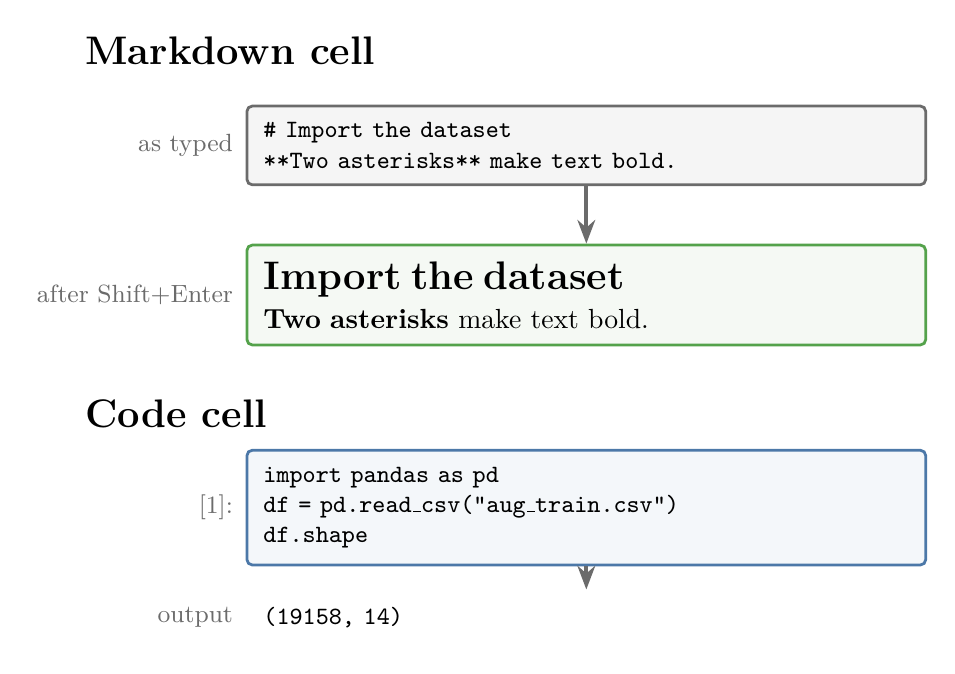
\begin{tikzpicture}[cell/.style={draw=#1, line width=1pt, rounded corners=2pt, text width=8.2cm, inner sep=6pt, align=left},
  tag/.style={font=\sffamily\small, text=cgrey, anchor=east}]
  \node[title, anchor=west] at (-2.3, 1.2) {Markdown cell};
  \node[cell=cgrey, fill=black!4, font=\ttfamily\small] (m1) at (4.2, 0) {\# Import the dataset\\{}**Two asterisks** make text bold.};
  \node[tag] at (-0.15, 0) {as typed};
  \node[cell=cgreen, fill=cgreen!6] (m2) at (4.2, -1.9) {{\sffamily\bfseries\Large Import the dataset}\\[2pt]{\sffamily \textbf{Two asterisks} make text bold.}};
  \node[tag] at (-0.15, -1.9) {after Shift+Enter};
  \draw[arrow] (m1.south) -- (m2.north);
  \node[title, anchor=west] at (-2.3, -3.4) {Code cell};
  \node[cell=cblue, fill=cblue!6, font=\ttfamily\small] (c1) at (4.2, -4.6) {import pandas as pd\\df = pd.read\_csv("aug\_train.csv")\\df.shape};
  \node[tag] at (-0.15, -4.6) {[1]:};
  \node[cell=white, font=\ttfamily\small] (c2) at (4.2, -6.0) {(19158, 14)};
  \node[tag] at (-0.15, -6.0) {output};
  \draw[arrow] (c1.south) -- (c2.north);
\end{tikzpicture}
\end{document}
